
\subsection{Vista lógica}

Se define los objetos, su estructura y sus relaciones con el resto de objetos.
De esta forma se explica cómo se realizan las funcionalidades descritas en la 
vista de casos de uso llevadas a cabo por medio de objetos. 

\subsubsection{Diagrama de clases generales}

\begin{figure}[H]
	\centering
 	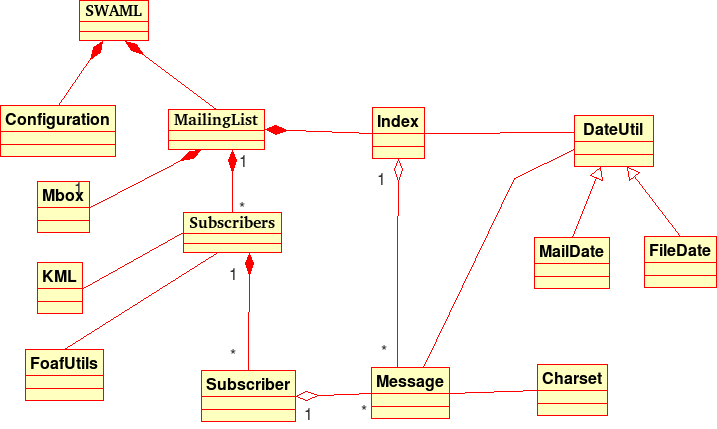
\includegraphics[width=15cm]{images/uml/clases/swaml.png}
	\caption{Diagrama de clases de SWAML}
	\label{fig:uml:swaml}
\end{figure}

\begin{figure}[H]
	\centering
 	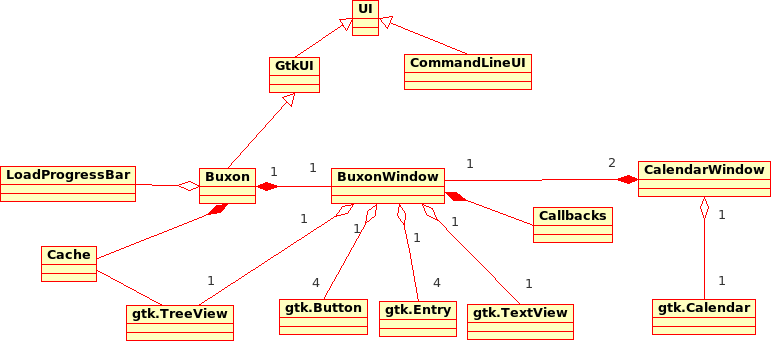
\includegraphics[width=17cm]{images/uml/clases/buxon.png}
	\caption{Diagrama de clases de Buxon}
	\label{fig:uml:buxon}
\end{figure}

\subsubsection{Detalle de las clases}

\paragraph{Clase SWAML:}

Implementa el punto de entrada a SWAML.

\begin{figure}[H]
	\centering
 	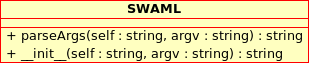
\includegraphics[width=7cm]{images/uml/clases/swaml-class.png}
	\caption{Detalle de la clase SWAML}
	\label{fig:uml:swaml-class}
\end{figure}

\paragraph{Clase UI:}

Clase (pseudo) abstracta que deben implementar los distintos interfaces de
usuario.

\begin{figure}[H]
	\centering
 	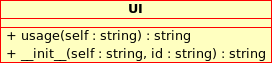
\includegraphics[width=6cm]{images/uml/clases/ui-class.png}
	\caption{Detalle de la clase UI}
	\label{fig:uml:ui-class}
\end{figure}

\paragraph{Clase CommandLineUI:}

Clase que implementa las funcionalidades básica necesarias para una aplicación
de consola.

\begin{figure}[H]
	\centering
 	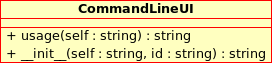
\includegraphics[width=6cm]{images/uml/clases/commandlineui-class.png}
	\caption{Detalle de la clase CommandLineUI}
	\label{fig:uml:commandlineui-class}
\end{figure}

\paragraph{Clase GtkUI:}

Clase que implementa alguno de los métodos usado en una interfaz de usuario
gráfica.

\begin{figure}[H]
	\centering
 	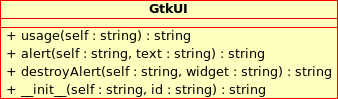
\includegraphics[width=7cm]{images/uml/clases/gtkui-class.png}
	\caption{Detalle de la clase GtkUI}
	\label{fig:uml:swaml-class}
\end{figure}

\paragraph{Clase MailingList:}

Abstracción de una lista de correo.

\begin{figure}[H]
	\centering
 	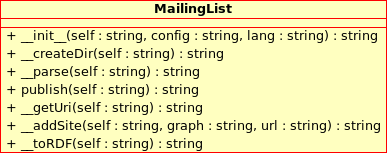
\includegraphics[width=9cm]{images/uml/clases/mailinglist-class.png}
	\caption{Detalle de la clase MailingList}
	\label{fig:uml:mailinglist-class}
\end{figure}

\paragraph{Clase Mbox:}

Clase encargada de gestiona la capa de acceso al mailbox.

\begin{figure}[H]
	\centering
 	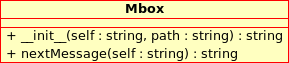
\includegraphics[width=6cm]{images/uml/clases/mbox-class.png}
	\caption{Detalle de la clase Mbox}
	\label{fig:uml:mbox-class}
\end{figure}

\paragraph{Clase Configuration:}

Clase encargada de la gestión de todos los parametros relacionados con la
configuración de la aplicación.

\begin{figure}[H]
	\centering
 	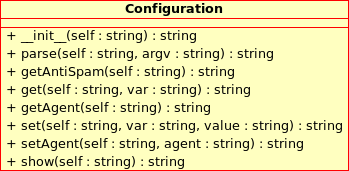
\includegraphics[width=8cm]{images/uml/clases/configuration-class.png}
	\caption{Detalle de la clase Configuration}
	\label{fig:uml:configuration-class}
\end{figure}

\paragraph{Clase Index:}

Clase encargada de gestionar toda la relación de indices (mensajes, suscriptores,
etc).

\begin{figure}[H]
	\centering
 	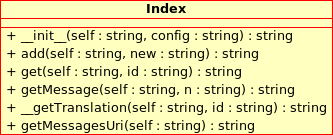
\includegraphics[width=7cm]{images/uml/clases/index-class.png}
	\caption{Detalle de la clase Index}
	\label{fig:uml:index-class}
\end{figure}

\paragraph{Clase Subscriber:}

Contenedor de suscriptores.

\begin{figure}[H]
	\centering
 	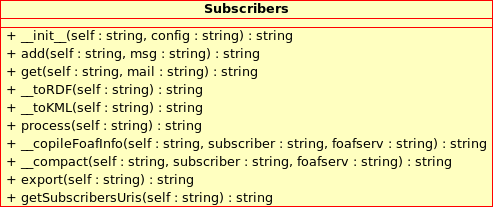
\includegraphics[width=10cm]{images/uml/clases/subscribers-class.png}
	\caption{Detalle de la clase Subscribers}
	\label{fig:uml:subscribers-class}
\end{figure}

\paragraph{Clase Subscriber:}

Abstracción de un suscriptor a una lista de correo.

\begin{figure}[H]
	\centering
 	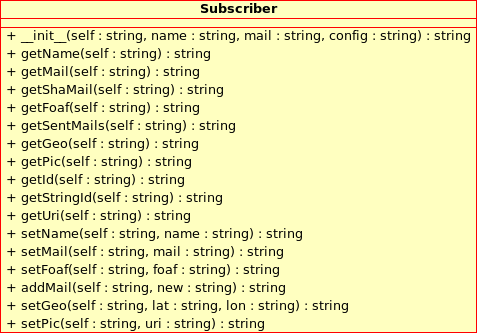
\includegraphics[width=10cm]{images/uml/clases/subscriber-class.png}
	\caption{Detalle de la clase Subscriber}
	\label{fig:uml:subscriber-class}
\end{figure}

\paragraph{Clase Message:}

Clase para describir un mensaje de correo electrónico.

\begin{figure}[H]
	\centering
 	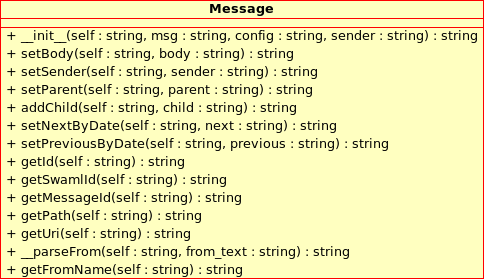
\includegraphics[width=10cm]{images/uml/clases/message-class.png}
	\caption{Detalle de la clase Message}
	\label{fig:uml:message-class}
\end{figure}

\paragraph{Clase DateUtil:}

Clase que engloba determinadas utilidades relacionadas con las fechas.

\begin{figure}[H]
	\centering
 	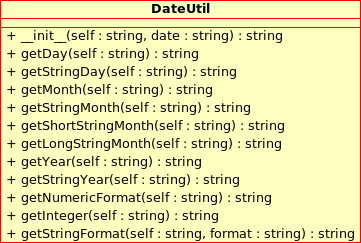
\includegraphics[width=8cm]{images/uml/clases/dateutil-class.png}
	\caption{Detalle de la clase DateUtil}
	\label{fig:uml:dateutil-class}
\end{figure}

\paragraph{Clase MailDate:}

Especialización de DateUtil para fechas en las cabeceras de correos electrónicos.

\begin{figure}[H]
	\centering
 	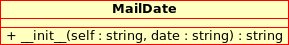
\includegraphics[width=6cm]{images/uml/clases/maildate-class.png}
	\caption{Detalle de la clase MailDate}
	\label{fig:uml:maildate-class}
\end{figure}

\paragraph{Clase FileDate:}

Especialización de DateUtil para trabajar con las fechas de ficheros.

\begin{figure}[H]
	\centering
 	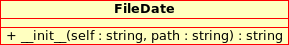
\includegraphics[width=6cm]{images/uml/clases/filedate-class.png}
	\caption{Detalle de la clase FileDate}
	\label{fig:uml:filedate-class}
\end{figure}

\paragraph{Clase Charset:}

Utilidades relacionadas para trabajar con distintas codificaciones de caracteres.

\begin{figure}[H]
	\centering
 	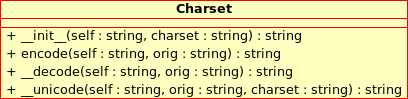
\includegraphics[width=8cm]{images/uml/clases/charset-class.png}
	\caption{Detalle de la clase Charset}
	\label{fig:uml:charset-class}
\end{figure}

\paragraph{Clase FoafUtils:}

Algunas utilidades para trabajar contra ficheros FOAF.

\begin{figure}[H]
	\centering
 	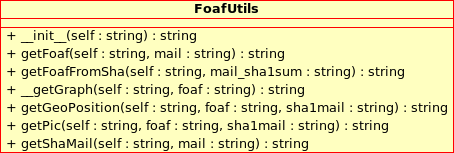
\includegraphics[width=9cm]{images/uml/clases/foafutils-class.png}
	\caption{Detalle de la clase FoafUtils}
	\label{fig:uml:foafutils-class}
\end{figure}

\paragraph{Clase KML:}

Pequeña biblioteca para trabajar con el formato KML de Google.

\begin{figure}[H]
	\centering
 	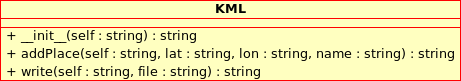
\includegraphics[width=10cm]{images/uml/clases/kml-class.png}
	\caption{Detalle de la clase KML}
	\label{fig:uml:kml-class}
\end{figure}

\paragraph{Clase Place:}

Abstracción de un punto geográfico para pintarlo en un fichero KML.

\begin{figure}[H]
	\centering
 	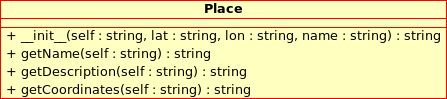
\includegraphics[width=10cm]{images/uml/clases/place-class.png}
	\caption{Detalle de la clase Place}
	\label{fig:uml:place-class}
\end{figure}

\paragraph{Clase Buxon:}

Clase maestra del visor Buxon.

\begin{figure}[H]
	\centering
 	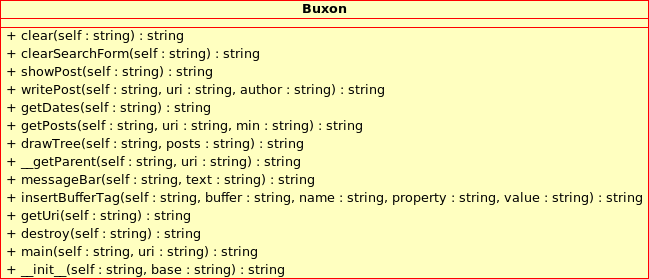
\includegraphics[width=13cm]{images/uml/clases/buxon-class.png}
	\caption{Detalle de la clase Buxon}
	\label{fig:uml:buxon-class}
\end{figure}

\paragraph{Clase BuxonMain:}

Punto de entrada para Buxon.

\begin{figure}[H]
	\centering
 	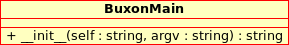
\includegraphics[width=6cm]{images/uml/clases/buxonmain-class.png}
	\caption{Detalle de la clase BuxonMain}
	\label{fig:uml:place-class}
\end{figure}

\paragraph{Clase Callbacks:}

Clase controlador de todas las señales que maneja Buxon.

\begin{figure}[H]
	\centering
 	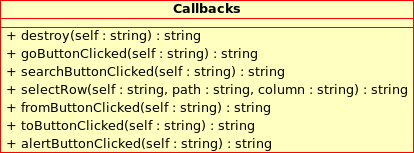
\includegraphics[width=9cm]{images/uml/clases/callbacks-class.png}
	\caption{Detalle de la clase Callbacks}
	\label{fig:uml:callbacks-class}
\end{figure}

\paragraph{Clase Cache:}

Clase que cachea un grafo de sioc:Forum.

\begin{figure}[H]
	\centering
 	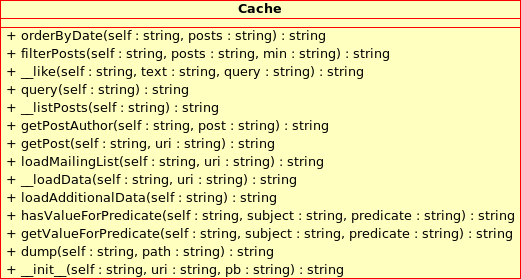
\includegraphics[width=11cm]{images/uml/clases/cache-class.png}
	\caption{Detalle de la clase Cache}
	\label{fig:uml:cache-class}
\end{figure}

\paragraph{Clase LoadprogressBar:}

Barra de progreso para procesos de carga.

\begin{figure}[H]
	\centering
 	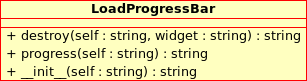
\includegraphics[width=7cm]{images/uml/clases/loadprogressbar-class.png}
	\caption{Detalle de la clase LoadProgressBar}
	\label{fig:uml:loadprogressbar-class}
\end{figure}

\paragraph{Clase CalendarWindow:}

Ventana de tipo popup con un calendario para simular la existencia de un
botón calendario.

\begin{figure}[H]
	\centering
 	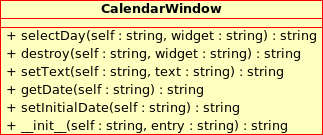
\includegraphics[width=7cm]{images/uml/clases/calendarwindow-class.png}
	\caption{Detalle de la clase CalendarWindow}
	\label{fig:uml:calenarwindow-class}
\end{figure}

\paragraph{Clase SwamlFoafEnricher:}

Interfaz para enriquecer suscriptores de SWAML usando FOAF.

\begin{figure}[H]
	\centering
 	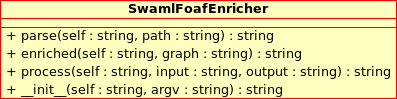
\includegraphics[width=9cm]{images/uml/clases/swamlfoafenricher-class.png}
	\caption{Detalle de la clase SwamlFoafEnricher}
	\label{fig:uml:swamlfoafenricher-class}
\end{figure}

\paragraph{Clase SwamlKmlExporter:}

Abstracción de un punto geográfico para pintarlo en un fichero KML.

\begin{figure}[H]
	\centering
 	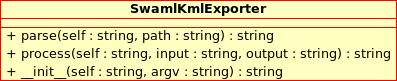
\includegraphics[width=9cm]{images/uml/clases/swamlkmlexporter-class.png}
	\caption{Detalle de la clase SwamlKmlExporter}
	\label{fig:uml:swamlkmlexporter-class}
\end{figure}
